\documentclass[../../main.tex]{subfiles}
\begin{document}
	\tableofcontents
	\newpage
	\section*{Introduction}
		Oldschool Runescape is a MMORPG which features combat. In combat, players are awarded experience for damage dealt to their opponents (often called monsters). After a certain amount of experience is gained the player may level up, improving the abilities in combat. The mechanics of combat involve accuracy, maximum damage, attack speed, among other details. There have been several attempts to quantify the experience rates according to a player's, and their opponent's levels and equipment. Although they are quite accurate, there are additional corrections that can be applied. Additionally extensions to more complex fighting scenarios has not been performed. We will be specifically considering applications to the Nightmare Zone, a common method of training combat. This game is played with long term investments and considerations in mind, as many achievements are achieved over periods of months or even years. In this sense, even minor optimizations can result in real-world savings for the player. Furthermore, the codebase that accompanies this article can be found at: \url{https://github.com/Palfore/OSRS-Combat}. This allows for more advanced use of the derived formulas (such as in optimization problems).

	\part{Modeling Combat}
		\chapter{Basics}
	% \section{Summary}
		The \href{https://oldschool.runescape.wiki/w/Maximum_hit}{official Wiki page} provides a very good review of maximum hit mechanics. For completion we will provide a brief summary. For some reason, it does not contain information about accuracy calculations. These are can be found (unofficially) from \href{https://www.osrsbox.com/blog/2019/01/22/calculating-melee-dps-in-osrs/}{osrsbox} (which references \href{https://docs.google.com/spreadsheets/d/1wzy1VxNWEAAc0FQyDAdpiFggAfn5U6RGPp2CisAHZW8/edit#gid=158500257}{DPS calculator by Bitterkoekje}, the \href{https://web.archive.org/web/20190905124128/http://webcache.googleusercontent.com/search?q=cache:http://services.runescape.com/m=forum/forums.ws?317,318,712,65587452}{forum post} of which has been archived), \href{https://www.reddit.com/r/2007scape/comments/40bvk6/accuracy_and_exphr_combat_formula/}{MachOSRS} (reddit), and \href{https://www.reddit.com/r/2007scape/comments/5lrty0/math_inside_corrected_accuracy_formula/}{[deleted]} (reddit).  Following this, we will take care to accurately determine the number of hits required to kill an opponent, followed by experience rate calculations. Related calculations have been performed by \href{https://www.reddit.com/r/2007scape/comments/4d6l7j/effects_of_overkill_on_dps/}{Nukelawe}, which discusses the impact of overkill on expected damage, which is often neglected in damage calculations. However we will justify that the application of this formula is not properly accounted for and we will instead provide an more accurate method.
		\section{Maximum Hit}
			There are three combat styles in the game: melee, ranged, and magic. The former two are quite similar, while the latter is slightly more involved. In general, there are 5 bonuses that a player can obtain to boost their maximum hit. These are bonuses from: potions, prayer, other, style, and special attack. These will be referred to as: $B^\text{pot}$, $B^\text{pray}$, $B^\text{other}$, $B^\text{style}$, $B^\text{SA}$, respectively. For non-magic styles, an effective damage level is defined as
			\begin{align}
				L^\text{eff} \equiv \left \lfloor \left(L + B^\text{pot} \right)B^\text{pray}B^\text{other} \right \rfloor + B^\text{style},
			\end{align}
			where $L$ is either the ranged level or strength level. The base damage, $D^\text{base}$ is then given by,
			\begin{align}
				D^\text{base} = C_0 + C_1S^\text{eff} + C_2 E^\text{str} + C_3 E^\text{str}S^\text{eff},\\
				\text{where}\,\,\, \{C\} = \left\{1.3, \frac{1}{10}, \frac{1}{80}, \frac{1}{640}\right\},
			\end{align}
			and $E^\text{str}$ is the ranged or melee strength bonus of the worn equipment. The max hit, $M$ is then given by,
			\begin{align}
				\boxed{M = \left \lfloor D^\text{base} B^\text{SA}\right \rfloor,}
			\end{align}
			where $B^\text{SA} = 1$ if no special attack is being used.

 			For melee, the \texttt{Keras} and \texttt{Saradomin Sword} are exceptions to this (see the wiki). For ranged, it should be noted that \texttt{bolt} effects only have probabilities of activating (and therefore increasing $M$). For future considerations, this could be handled by defining an effective or average max hit: $\langle M \rangle = P M$, where $P$ is the probability of activation. Additionally, some sources state that some equipment which would be categorized under ``other'' bonuses such as the \texttt{Slayer helmet} actually use $\left \lfloor D^\text{base} B^\text{SA}B^\text{other}\right \rfloor$ and so act as a multiplier instead of its expected placement. This is not stated on the wiki, but appears to be correct.
			\subsubsection{Magic}
				The base damage for a magic spell is fixed and only multiplicative bonuses are obtainable. A single bonus yields a max hit of,
				\begin{align}
					M = D^\text{base}E^\text{str},
				\end{align}
				where now $E^\text{str}$ is the multiplicative magic damage bonus (think ``magic strength''). In general, these effects stack, but intermediate flooring calculations can impact the max hit (check the wiki for ordering). \texttt{Charge}, \texttt{Magic dart}, \texttt{Salamanders}, and \texttt{Trident of the seas/swamp} have alternate calculations.
		\section{Accuracy}
			$A$ will denote the player's probability of a successful hit (called accuracy). This attribute depends on both the player and the opponents stats. For all three combat styles, the attacker rolls an attack role, while the defender rolls a defensive roll. First effective levels are calculated,
			\begin{align}
				L^\text{eff}_A \equiv \left \lfloor \left(L + B^\text{pot} \right)B^\text{pray}B^\text{other} \right \rfloor + B^\text{style} + 8,
			\end{align}
			where the subscript on $L_A$ is used to denote the difference between the effective damage levels discussed above, and these effective accuracy levels.
			Then the maximum roll is given by,
			\begin{align}
				R_\text{max} = \left \lfloor L_A^\text{eff} (E + 64)\right \rfloor,
			\end{align}
			where $E$ is the equipment bonus for the respective attack or defense style.
			Now the accuracy is given according to,
			\begin{empheq}[box=\fbox]{align}
				a = \begin{cases}
					1 - \frac{1}{2}\frac{D_\text{max} + 2}{A_\text{max} + 1} & A_\text{max} \ge D_\text{max} \\
					\frac{A_\text{max}}{2D_\text{max} + 2} & \text{else},
				\end{cases}
			\end{empheq}
			where $A_\text{max}$ and $D_\text{max}$ represent the maximum attack and defense rolls ($R_\text{max}$) respectively. This is plotted in Fig.~\ref{fig:accuracy}. No information suggests magic accuracy is any different. No other work / official statements show how special attacks factor into this. It is a fair assumption that $a^\text{eff} = aB^\text{SA}$ for special attacks that increase accuracy (since no flooring needs to be done for accuracy).
			\begin{figure}[H]
				\centering
				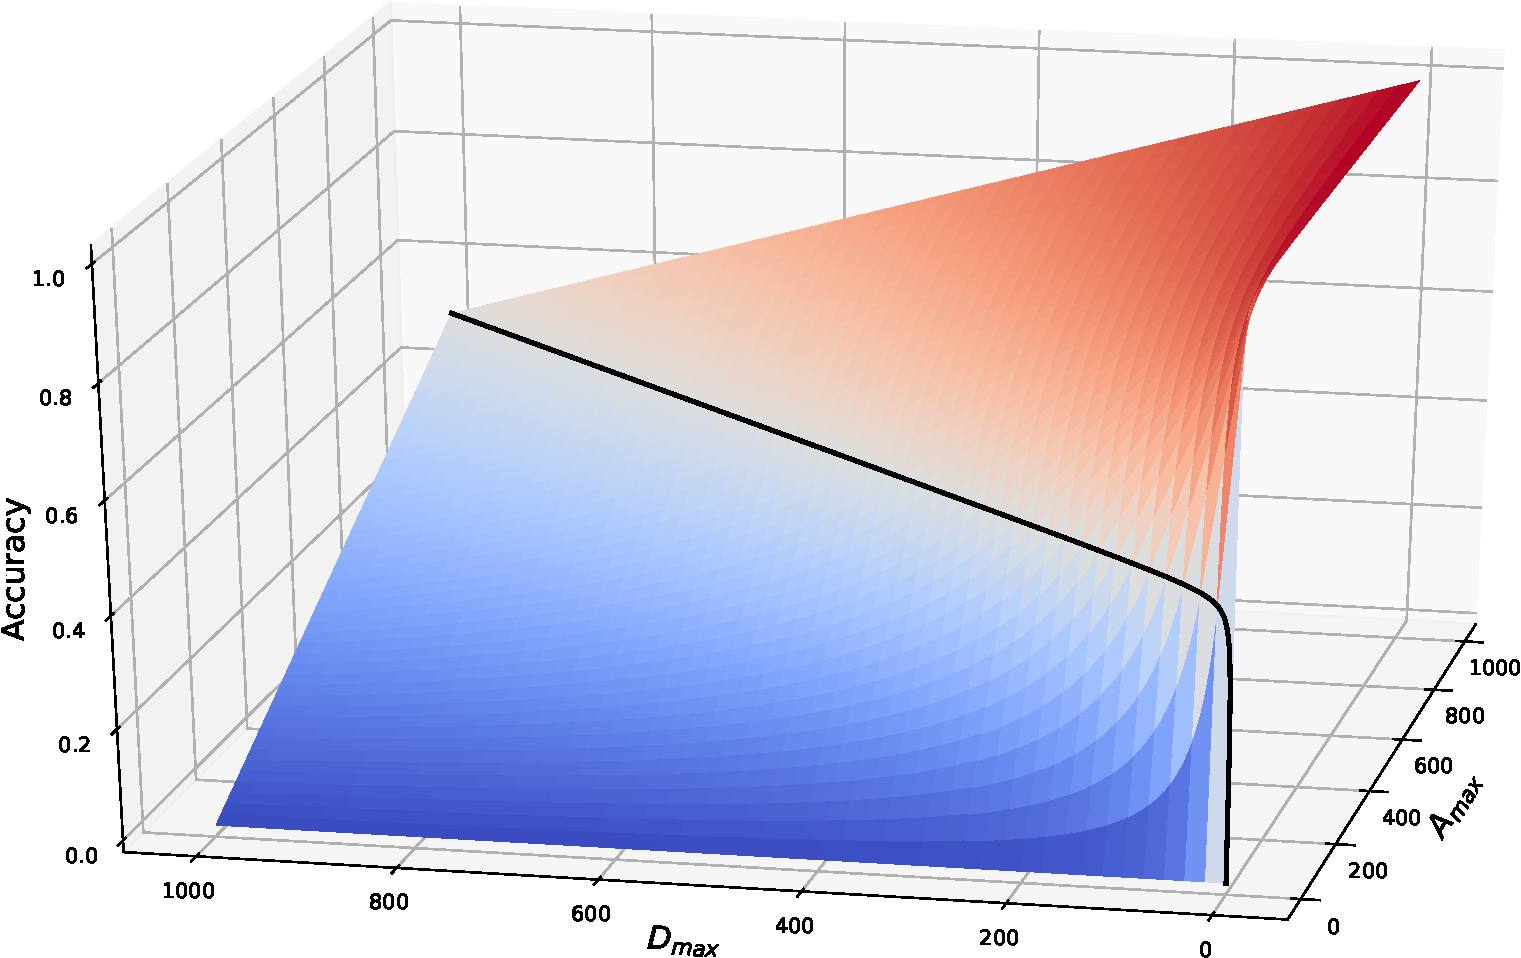
\includegraphics[width=\linewidth]{../Code/osrsmath/results/part_I/Accuracy.pdf}
				\caption{Player accuracy as a function of the player's maximum accuracy roll and opponent's maximum defense roll. The black line is the piecewise boundary.}
				\label{fig:accuracy}
			\end{figure}

		\section{Experience and Damage Per Second}
			In the next chapter, we will look at modeling the number of turns, $n$ to kill an opponent. The time to kill is simply $T_An/a$ where $T_A$ is the time between attacks. Experience is calculated as a multiple, $e$ of the damage done. So the experience per second is given by,
			\begin{equation}
				\boxed{E=\frac{eah_0}{T_An}}
			\end{equation}
			noting that $n$ is also a function of $h_0$, so $E$ does \emph{not} increase linearly with $h_0$. For most opponents, $e=4$. However there are \href{https://twitter.com/BitterkoekjeRS/status/803960032178110468}{exceptions}.



	\chapter{Models}
		There are several models that can used to model combat. They vary in how they handle overkill and they will be presented roughly in order of increasing accuracy. These models operate on the following assumptions:
		\begin{enumerate}
			\item A successful attack is uniformly distributed between $[0, M]$ (noting there are $M+1$ integers in this range).
			\item An attack is successful with the probability $a\in[0, 1]$, which is the attacker's accuracy.
			\item The defender starts at a health $h_0$.
			\item Attacks occur every $T_A$ seconds.
			\item No special attacks, or weapon switches are considered.
			\item The first attack occurs at time, $t=0$ or attack number $n=0$ depending on context.
			\item If health regeneration is considered, it occurs every $T_r$, and heals one health.
					The first regeneration will occur as a uniform random variable at $t\sim U[0, T_r]$.
		\end{enumerate}
		There are two relevant quantities that will be calculated for each model: time to health, and health after time.

		There are some basic results we can already state:
		\begin{enumerate}
			\item The number of attack attempts is simply $a$ times the number of successful attacks.
			\item The time taken for $n$ attacks is simply $nT_A$.
		\end{enumerate}

		Only the last model will discuss health regeneration, and it will take a non-regeneration model as input so it applies generally.
		Finally, a comparison between the different models will be performed.

		\section{Crude Model}
			\subsection{Health after $n$ attacks}
				This model does not consider overkill and as a result is very straight forward. The average damage per successful attack is,
				\begin{align}
					\langle D \rangle &= \frac{1}{M+1}\sum_{i=0}^M i\\
						&= \frac{1}{\cancel{M+1}} \frac{M\cancel{(M+1)}}{2}\\
						&= \frac{M}{2}.
				\end{align}
				After each attack, the health will lower by this amount, recursively this allows us to state:
				\begin{equation}
					h_{n+1} = h_{n} - \langle D \rangle,\,\,\,h_0\equiv\text{Initial Health}.
				\end{equation}
				In this case the health after $n$ successful attacks is:
				\begin{align}
					h_{n+1} &= h_{n} - \frac{M}{2}\\
					\Aboxed{h_{n} &= h_0 - n\frac{M}{2}}.
				\end{align}
			\subsection{Attacks until $h$ health}
				This equation can be inverted to give the number of turns to a given health,
				\begin{align}
					\Aboxed{n &= (h_0 - h_{n}) \frac{2}{M}}.
				\end{align}
				Both of these can be calculated in $\mathcal{O}(1)$ time.
		\section{Nukelawe}
			\subsection{Health after $n$ attacks}
				\href{https://imgur.com/aykEahg}{Nukelawe} presents a derivation that gives the average damage per hit over the opponent's life to be,
				\begin{align}
					\langle D \rangle_{h_0}^M = \frac{y(y+1)}{h_0(M+1)}\left(\frac{1}{2}{(M+h_0+1)}-\frac{1}{3}(2y+1) \right),
				\end{align}
				where $y=\min(h_0, M)$. This makes use of an average over a piecewise function which is an approximation. The Recursive model removes this assumption. However this allows the average damage to be independent of the current health, allowing us to get a similar solution to the Crude case,
				\begin{align}
					\Aboxed{h_{n} &= h_0 - n\frac{y(y+1)}{h_0(M+1)}\left(\frac{1}{2}{(M+h_0+1)}-\frac{1}{3}(2y+1) \right)}.
				\end{align}

			\subsection{Attacks until $h$ health}
				And again, inverting and simplifying a bit, we get,
				\begin{align}
					\Aboxed{n &= \frac{6h_0(M+1)(h_0 - h_{n})}{ y(y+1)\left(2(M+h_0+1)-2(2y+1) \right)} }.
				\end{align}
				Both of these can be calculated in $\mathcal{O}(1)$ time.

		\section{Recursive Model}\label{sec:average_damage}
			\subsection{Expected Damage per Hit}
				The Crude model made the assumption that the player can always hit up to their max hit. This is not the case if the opponent has less health, $h$ than the maximum hit.
				\begin{center}
				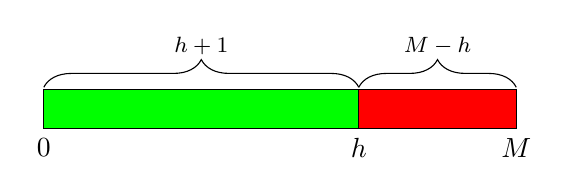
\begin{tikzpicture}
					\filldraw[fill=green, draw=black] (0,0) node[anchor=north] {$0$} -- (4,0) node[anchor=north] {$h$} -- (4,0.5) -- (0,0.5) -- (0,0);
					\filldraw[fill=red, draw=black] (4,0) -- (6,0) node[anchor=north] {$M$} -- (6,0.5) -- (4,0.5) -- (4,0);
					\draw [decorate,decoration={brace,amplitude=10pt},xshift=0pt,yshift=15pt]
					(0,0) -- (4,0) node [black,midway,yshift=15pt]{
						\footnotesize $h+1$
					};
					\draw [decorate,decoration={brace,amplitude=10pt},xshift=0pt,yshift=15pt]
					(4,0) -- (6,0) node [black,midway,yshift=15pt]{
						\footnotesize $M-h$
					};
				\end{tikzpicture}
				\end{center}
				Considering this, we could hit every integer below $h$ each with a probability of $1/(M+1)$, and we could hit exactly $h$ (since we're considering hits capped by $h$) with a probability of $(M-h)/(M+1)$. Averaging the expectations gives,
				\begin{align}
					\langle D \rangle_{h < M} &= \frac{1}{M+1}\sum_{i=0}^{h} i + \frac{M-h}{M+1}h \\
					&= \frac{1}{M+1}\frac{h(h+1)}{2} + \frac{M-h}{M+1}h \\
					&= \frac{h}{2}\frac{2M-h+1}{M+1}\\
					&= \frac{h}{2}\left(1 + \frac{M - h}{M+1}\right)\\
					&= \frac{h}{2}\left(2 - \frac{h + 1}{M+1}\right)
					% &= \frac{h^2}{2m} + \frac{h}{2m} + h - \frac{h^2}{m} \\
					% &= -\frac{h^2}{2m} + \left(\frac{1}{2m} + 1\right)h \\
				\end{align}

				Overall then, our expected damage on a successful hit is:
				\begin{align}
					\boxed{
						\langle D \rangle = \frac{1}{2}\begin{cases}
							M &\text{if $h \ge M$} \\
							h\left(2 - \frac{h + 1}{M+1}\right) &\text{if $h < M$} \\
						\end{cases}
					}
				\end{align}

				\begin{figure}
					\centering
					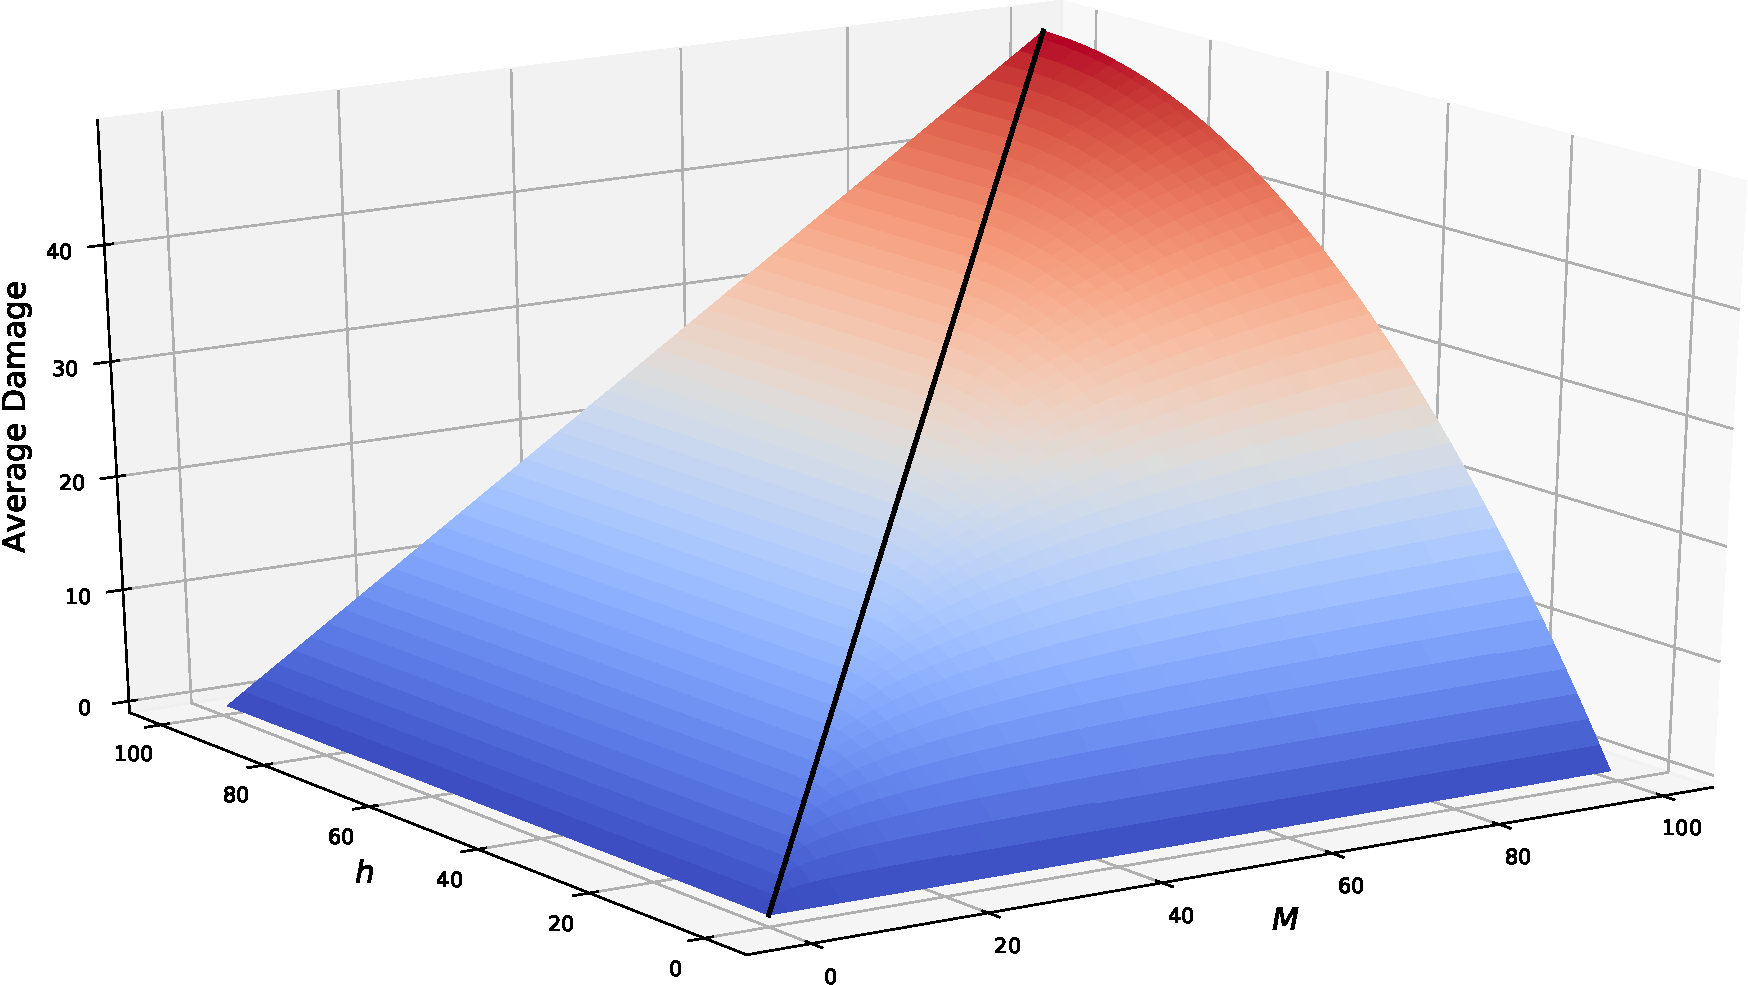
\includegraphics[width=\linewidth]{../Code/osrsmath/results/part_II/average_damage.pdf}
					\caption{The average damage of an attack with a maximum hit of $M$ on an opponent with $h$ health. The black line is the piecewise boundary.}
					\label{fig:average_d}
				\end{figure}


				This is plotted in Fig.~\ref{fig:average_d}. The Nukelawe model averages over these contributions for the \emph{overall} (i.e. not piecewise) expected hit, assuming each starting health is equally likely. This isn't totally accurate, regardless, it is good to check that our equations agree under this assumption:
				\begin{align}
					\langle D \rangle_\text{overall} &= \left \langle \langle D \rangle_{h < M} + \langle D\rangle_{h\ge M} \right \rangle\\
					&= \frac{1}{h_0}\left(\sum_{h<M} \langle D \rangle_{h < M} + \sum_{h\ge M}\langle D\rangle_{h\ge M} \rangle \right)\\
					&= \frac{1}{h_0}\left(
						\sum_{n=M+1}^{h_{0}}\frac{M}{2} +
						\sum_{n=1}^{y} \frac{n}{2}\left(2 - \frac{n + 1}{M+1}\right)
					\right) \\
					&= \frac{y(y+1)}{h_0(M+1)}\left(\frac{1}{2}{(M+h_0+1)}-\frac{1}{3}(2y+1) \right),
				\end{align}
				where $y=\min(M, h_0)$. The last step is actually quite tricky and involved to show. For that reason it can be found in Appendix~\ref{app:average_damage}. This agrees with Nukelawe's findings.

			\subsection{Health after $n$ attacks}
				Despite the above being an ``average'', it is not the average damage expected per hit over the life time of an opponent since certain healths are much more likely to appear than others. As an example, suppose there is an opponent with 100 health fighting an attacker with a max hit of 30. On the first hit, the most likely health is 85. This means that unlike the above calculation, each hit is \emph{not} equally likely. Particularly, this over estimates the contribution in the overkill region, since (depending on the circumstances) let's say 1 or 2 hits is expected per kill. Those 1 or 2 hits are more likely to occur at specific $h$ values, but the average sums across all $h$ equally. In the non-overkill region, this has no impact due to it being constant. The proper treatment is to use the piecewise damage expectation in the recursive definition:
				\begin{align}
					h_{n+1} = h_{n} - \frac{1}{2}\begin{cases}
						M &\text{if $h_n \ge M$} \\
						h_n\left(2 - \frac{h_n + 1}{M+1}\right) &\text{if $h_n < M$}.
					\end{cases}
				\end{align}
				This however is too cumbersome to handle at once. Since the health is a decreasing monotonic function, we can consider it in two parts. While $h$ is above or equal to $M$ the solution to the above is the same as the Crude model's,
				\begin{align}
					h_n = h_0 - n\frac{M}{2}.\label{eq:h_crude}
				\end{align}
				The solution to the other is a bit more complex. After a certain number of iterations the health will drop below $M$ and the second case above will kick in. We'll say this occurs after $L$ iterations (noting that this \emph{average} quantity can be a non-integer),
				\begin{align}
					M &> h_0 - L\frac{M}{2} \\
					\frac{2}{M}(h_0 - M) &< L \\
					\implies L &= 2\left(\frac{h_0}{M} - 1\right).
				\end{align}
				Now the expected health that the second condition starts at is given by,
				\begin{align}
					\langle h_L \rangle &= h_0 - 2\left(\frac{h_0}{M} - 1\right) \frac{M}{2}\\
					&= M.
				\end{align}
				Thus the second case is expected to starts on iteration $L$ with an initial health of $M$. For simplicity, we will define $m\equiv n-L$. Returning to our recursive function,
				\begin{align}
					h_{m+1} &= h_{m} - \frac{h_m}{2}\left(2 - \frac{h_m + 1}{M+1}\right) \\
					&= h_{m} - h_m + \frac{h_m}{2}\frac{h_m + 1}{M+1} \\
					&= \frac{h_m^2 + h_m}{2(M+1)} \\
					h_{m+1} &= \gamma (h_m^2 + h_m), \label{eq:recur}
				\end{align}
				where $\gamma\equiv1 / 2(M+1)$. This type of recurrence relation is called a \href{http://mathworld.wolfram.com/QuadraticMap.html}{Quadratic Map}, and unfortunately it has no closed form solution in general. Some work is shown in Appendix~\ref{app:analytic_form_attempt} to attempt to simplify it, but no final form was realized. For the sake of completeness, we will call the solution to Eq.~\ref{eq:recur} $f(m; M, f_0)$. At this point we're left with,
				\begin{align}
						h(n; h_0, M) &=  \begin{cases}
						h_0 - \frac{1}{2}nM &\text{else if $n \le L$} \\
						f(n - L; M, M) &\text{otherwise}.
					\end{cases}
				\end{align}

				In general, we are more interested in the number of iterations that is required to kill an opponent which is the inverse of this function, $n=h^{-1}(h; h_0, M)$. However, since the recurrence relation cannot be solved analytically, we cannot obtain a general expression for this. We could numerically compute this result. However remember that we are dealing with \emph{expectation values} or averages. This means it is totally possible for the inverted function to say ``The opponents health will be 18 in 4.5 iterations, on average''. This is a problem because our recursive equation can only increment the iteration by one (and we can only start at $f_0$)! In the next section, we will look at an approximation that will allow us to handle non-integer expectations.

		\subsubsection{Approximate Solution}
				Despite not being able to find a closed-form solution for Eq.~\ref{eq:recur}, we can look for approximate solutions. Although it's rare, there are a few quadratic recurrence relations that \textbf{do} have solutions. There are two relevant cases, ones where a constant term is introduced, or ones where the linear term is removed. Since increasing $n$ (and therefore iterations) results in smaller and smaller $h_n$, it suggests that adding constant terms will heavily skew the results in this region. Removing the linear term is still not ideal since its contribution increases relative to the quadratic term, in the low $h_n$ limit (when this recursive case is required). However this should be less significant and we'll find that it does pretty well! If this justification does not satisfy you, please check out Appendix~\ref{app:recursive_approximation_justification}. With this approximation, our recursive relation becomes,
				\begin{align}\label{eq:simplified_recursion}
					h_{m+1} = \gamma h_m^2.
				\end{align}
				Starting with $h_0 = M$, and looking at a few terms reveals,
				\begin{align}
					h_{1} &= \gamma^1 M^2\\
					h_{2} &= \gamma^1 h_1^2\\
						&= \gamma^1 \gamma^2 M^{(2\cdot2)}\\
					h_{3} &= \gamma^1 h_2^2\\
						&= \gamma^1 \gamma^2 \gamma^4 M^{(2\cdot2\cdot2)}\\
					\implies h_m &= \gamma^{\sum_{i=0}^{m-1} 2^i} M^{2^m}\\
								&= \gamma^{2^m-1} M^{2^m}\\
								&= \frac{1}{\gamma}(\gamma M)^{2^m}\\
							\Aboxed{h_m &= \frac{1}{\gamma}\left(\frac{1}{2} - \gamma\right)^{2^m}}
				\end{align}
				This equation is not only a closed form expression, but it can also be inverted!
				\begin{align}\label{eq:approximate_m}
					\log_2(\log_{\frac{1}{2} - \gamma} (\gamma h_m)) &= m.
				\end{align}
				This equation asymptotically reaches 0, but the opponent dying occurs when $h_m$ drops below 1 yielding an average kill on iteration,
				\begin{align}
					\log_2(\log_{\frac{1}{2} - \gamma} (\gamma)) &= m.
				\end{align}

				How can we make use of this approximation to improve our more accurate calculation? Remember that we are trying to solve the issue of non-integer iterations. Instead of beginning on iteration 0 for the iterative procedure, we can start $m$ at any real number in (0, 1), and iterate upwards on that. For example to get the health at iteration 4.87, we could use our analytic approximation to calculate 0.87 (which uses \textit{one} approximation), then iterate 4 times using the correct equation to get to the final result. So this defines our new best approximation,
				\begin{empheq}[box=\fbox]{align}\label{eq:recursive_h}
						h(n; h_0, M) &=  \begin{cases}
						h_0 - \frac{1}{2}nM &\text{if $n \le L$} \\
						\frac{1}{\gamma}\left(\frac{1}{2} - \gamma\right)^{2^{n-L}} &\text{if $n - L < 1$}\\
						f\left(n - L; M, \frac{1}{\gamma}\left(\frac{1}{2} - \gamma\right)^{2^{n-L}}\right) &\text{otherwise}\\
					\end{cases}\\
					\text{where, }\gamma = &\frac{1}{2(M+1)}\text{ and } L = 2\left(\frac{h_0}{M} - 1\right).\nonumber
				\end{empheq}

				\subsection{Attacks until $h$ health}
					To solve for when the opponents health drops below one, $n=h^{-1}(1)$, we must use a numerical root finding algorithm to solve for the zero of $(1 - h(n))$. It is possible that $h^{-1}(1/2)$ is more representative of death than $h^{-1}(1)$. However, empirically, using 1 is in better agreement with simulation.

					The time complexity can be approximated using Eq.~\ref{eq:approximate_m}:
					\begin{align}
						\mathcal{O} &= \log_2(\log_{\frac{1}{2} - \gamma} (\gamma h_m))\\
						  &\propto \log\left( \frac{\log(\gamma h_m)}{\log (\frac{1}{2} - \gamma)}\right)\\
						  &\approx \log\left( \frac{\log(\frac{1}{\gamma h_m})}{\log (2)}\right)\\
						  &= \log\log\left(\frac{1}{\gamma h_m}\right) - \log\log (2)\\
						  &\sim \log\log\left(\frac{1}{\gamma h_m}\right)\\
						  &\approx \log\log\left(\frac{2m}{h_m}\right).
					\end{align}
					Here, $\propto$ is used to signal a multiplicative factor was ignored, and $\sim$ is used to signal an additive factor was ignored. In the first line the change of base formula was used, and the factor $log(2)$ was ignored. In the second line, $1/2-\gamma\approx1/2$ was used. This leaves us with $\mathcal{O}(\log\log(2m/h))$ evaluations required, which is practically constant. However, the number of evaluations for the numerical inversion depends on the implementation. In practice, at most 30 evaluations are required.


		\section{Approximately Analytic Recursion}
			\subsection{Health after $n$ attacks}
				We can simplify the Recursive model by extending the approximation to all $n > L$:
				\begin{empheq}[box=\fbox]{align}
					h(n; h_0, M) &=  \begin{cases}
						h_0 - \frac{1}{2}nM &\text{if $n \le L$} \\
						\frac{1}{\gamma}\left(\frac{1}{2} - \gamma\right)^{2^{n-L}} &\text{otherwise}.
					\end{cases}
				\end{empheq}

			\subsection{Attacks until $h$ health}
				This is useful because it can be inverted analytically:
				\begin{empheq}[box=\fbox]{align}
					n(h; h_0, M) &=  \begin{cases}
						(h_0 - h) \frac{2}{M} &\text{if $h \ge M$} \\
						\log_2(\log_{\frac{1}{2}-\gamma}(\gamma h)) &\text{otherwise}
					\end{cases}.
				\end{empheq}
				These can be evaluated in $\mathcal{O}(1)$ time.


		% \section{Markov Chain}

		\section{Health Regeneration}
			We have a function $h(n; a, M, h_0)$ that models the health of the opponent after $n$ total attacks, without regeneration. Based on the weapon attack interval, $T_A$, we can convert to seconds through $t = nT_A$. This leaves us with $h(t/T_A; a, M, h_0)$. These equations cannot solve health regeneration since the health no longer decreases monotonically, and as a result the cases cannot be separated. Let's roll with this restriction and solve the problem within a window where the opponent does not heal. First we will make the assumption that the first regeneration occurs at $t=T_R$, which is the time between regenerations. We will later remove this restriction by averaging the first regeneration over $t\in[0, T_R]$. To reduce clutter, let's remove some explicit parameters and redefine $h$ as $h(t, h_0)$. The health just before the opponent heals is
			\begin{align}
				h_1 = h(T_R, h_{0}),
			\end{align}
			which is the health after $T_R$ seconds starting from some initial health $h_0$. Immediately after, the opponent will heal by $+1$ health,
			\begin{align}
				h_1 = h(T_R, h_{0}) + 1.
			\end{align}
			Iterating again:
			\begin{align}
				h_2 &= h(T_R, h_1) + 1 \\
					&= h(T_R, h(T_R, h_0) + 1) + 1.
			\end{align}
			Letting, $f(x)=h(T_R, x)$ to, again, reduce clutter and iterating again yields,
			\begin{align}
				h_3 &= f(h_2) + 1 \\
					&= f(f(h_1) + 1) + 1 \\
					&= f(f(f(h_0) + 1) + 1) + 1.
			\end{align}
			In general this gives us an \textit{iterated function},
			\begin{align}
				h_m &= g^{\circ m}(h_0),
			\end{align}
			where $m$ is the number of regeneration periods, and $g(x) \equiv f(x) + 1$. As an example of the function composition, for $m=2$ the above expands to:
			\begin{align}
				g^{\circ 2}(x)&=(g\circ g)(x)=g(g(x)) \\
							&=f(f(x) + 1) + 1.
			\end{align}
			This is great but this process doesn't continue indefinitely since the opponent will eventually die. There is a health, $h^*$ after which, the opponent will not be able to heal. Starting at a health of zero, we can determine how much health the player had $T_R$ seconds ago,
			\begin{align}
				h^* = h(-T_R, h_0=0)
			\end{align}
			Let's summarize. The opponent starts at $h_0$ health. They will not heal after $h^*$. The time taken to die is equal to the number of healing cycles until they drop below $h^*$. Plus the time it takes to get from that remaining health (not necessarily $h^*$) to 0. Pseudocode for this is given below, where \verb| health_after | and \verb| time_to_kill | are both non-regen functions. Parameters like accuracy and max hit are omitted.

			\begin{lstlisting}[language=Python, escapeinside={(*}{*)}]
def time_to_kill_regen(h_0):
	h = (*$h_0$*)
	t = 0
	(*$h^*$*) = health_after(-(*$T_R$*), 0)
	while h (*$\ge$*) (*$h^*$*):
		h = health_after((*$T_R$*), h) + 1
		t += (*$T_R$*)
	return t + time_to_kill(h)\end{lstlisting}


			Now consider the initial condition. We assumed that the first regeneration occurred at $T_R$. However, it is a discrete (due to game ticks) uniform random variable distributed between $t_r \sim U[1, T_R]$. If a tick occurs every $\tau$ seconds, then there are $T_R/\tau$ game ticks before a heal.
			\begin{align}
				h_1 &= h(t_r, h_0) \\
				h_2 &= h(T_R, h(t_r, h_0) + 1) \\
				h_3 &= h(T_R, h(T_R, h(t_r, h_0) + 1) + 1) \\
				h_n &= (h\circ (x+1))^{\circ n-1}(T_R, h(t_r, h_0)) \\
				\langle h_n \rangle &= \frac{\tau}{T_R}\sum_{i=1}^{T_R/\tau} (h\circ (x+1))^{\circ n-1}(T_R, h(i\tau, h_0))
			\end{align}
			Now this has to be numerically inverted to give the time to kill.

		\section{Comparisons}
			We have seen several methods for calculating expected kill iterations. We can now compare these models to numerically simulated fights as in Fig.~(\ref{fig:comparison}). Regardless of the model, the turns to kill grows quickly when the max hit is low compared to the initial health of the opponent (as expected). The models deviate the most from the simulations when the initial health is low, and when the max hit is high. Both the crude method and the Bitt-Nuke method have unbounded errors, while the Recursive method actually has a maximum near $(h, M) \approx (25, 80)$. Thus the recursive method is not only more accurate (less error), it also holds in more cases.
			%This is expected to improve accuracy by about 1-5\% depending on the fighters (remember that the benefit of this scales over periods of weeks \& months!).
			% For max melee, this saves 11 hours!

			\begin{figure}
				\centering
				\begin{subfigure}{.5\textwidth}
					\centering
					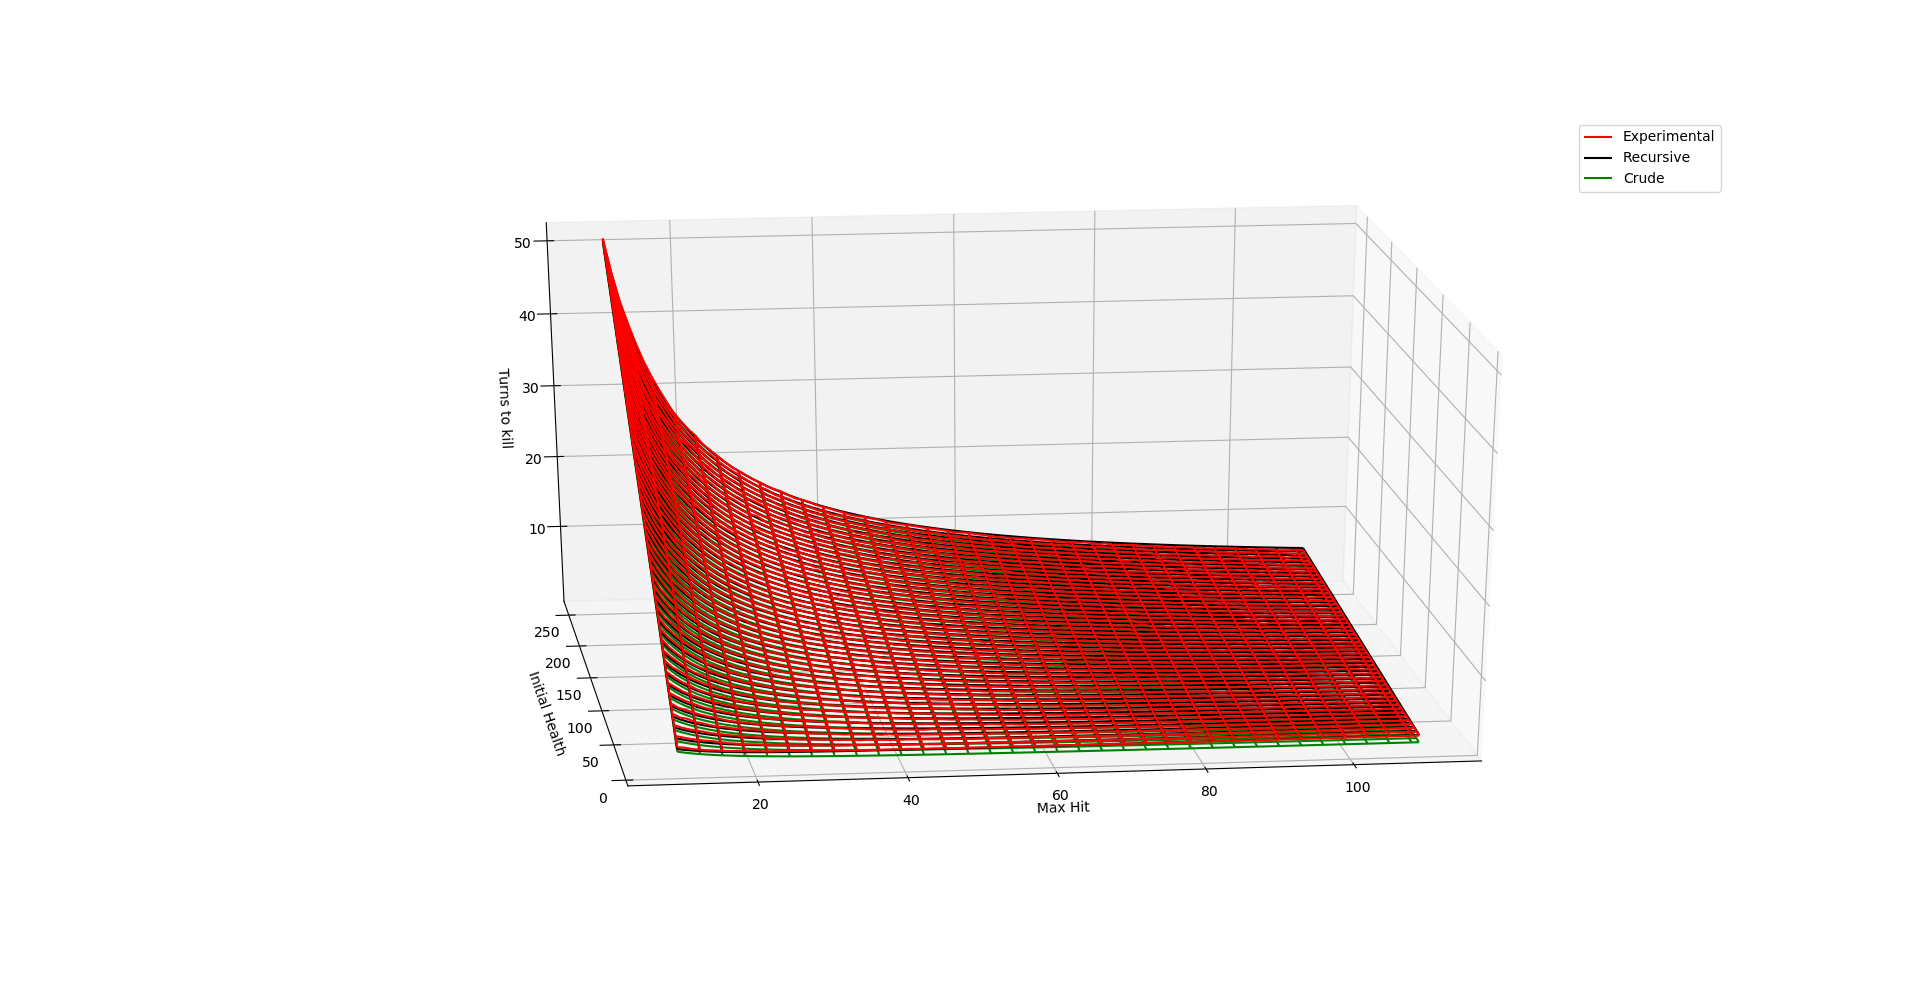
\includegraphics[width=\linewidth]{img/h2k_h2.png}
					\caption{Turns to Kill}
					% \label{fig:sub1}
				\end{subfigure}%
				\begin{subfigure}{.5\textwidth}
					\centering
					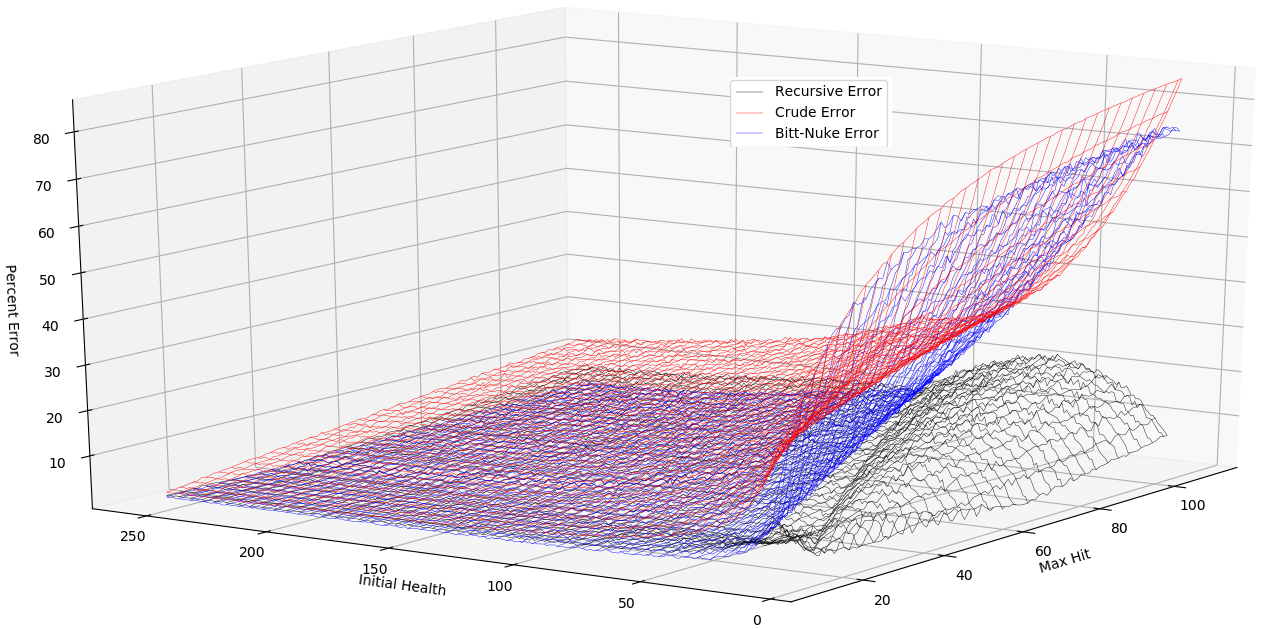
\includegraphics[width=\linewidth]{img/error.png}
					\caption{Error from Simulation}
					% \label{fig:sub2}
				\end{subfigure}
				\caption{
					A comparison between different models. The crude model does not consider the effects of overkill. The recursive model is that described in Eq.~\ref{eq:recursive_h} which best accounts for overkill. The Bitt-Nuke model averages the effect of overkill. The true value can be evaluated by simulating many fights and averaging the results. To get high precision this is a very expensive evaluation. On the left, the expected number of successful hits required for a kill is shown. All three models \textit{appear} quite similar, however this is an artifact of scale. On the right, the percent relative error with respect to the simulations are shown. The noise is evident and occurs due to the difficulty of efficiently simulating the required number of fights. The peak error is the region in which overkill is expected to occur. The average error of the recursive method is 4.94\% with a standard deviation of 4.8\%, while the Bitt-Nuke method has an average of 10.57\% and a standard deviation of 17.4\%.
				}\label{fig:comparison}
			\end{figure}


	\chapter{Nightmare Zone}
		We can now attempt to extend this into an useful application. For practical purposes, the Nightmare Zone (NMZ) is a combat training ground minigame that offers a low intensity, but efficient method of training combat skills. The player enters an arena with several bosses they have previously fought in the main game. At any given time, four (randomly chosen - with replacement) are in combat with the player. Before beginning, the player can decide a minimum of five bosses they would like to re-fight.

		\begin{figure}
			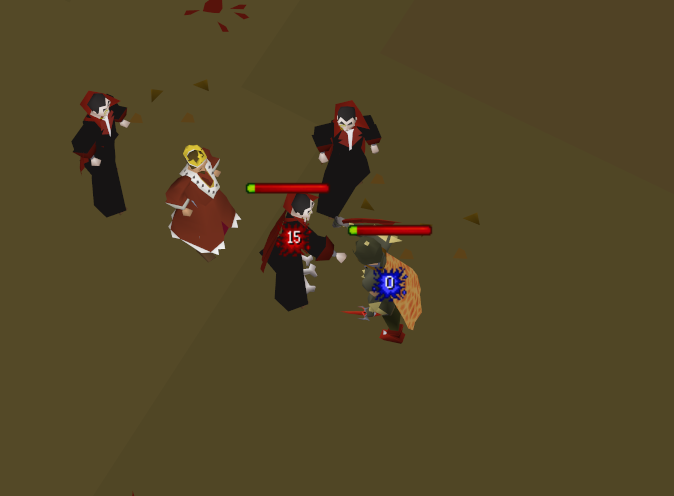
\includegraphics[width=\linewidth]{img/NMZ.png}
			\caption{A player (bottom-right) fighting against four bosses in the NMZ. Three of the bosses at this time happened to be the same, however each boss is expected to occur with equal probability.}
			\label{fig:nmz}
		\end{figure}

		This can be seen as a first a check, and second an optimization problem (to maximize experience). At this point we have calculated the experience per hour in terms of: accuracy, max hit, initial opponent health, and attack speed. The accuracy and max hit are involved yet straightforward calculations, while the other parameters are generally in a database. We have only made two assumptions so far, no health regeneration, and constant combat, along with 1 approximation in the turns to kill formula. \textcolor{red}{1 health is regenerated every minute the opponent is under their maximum health. [Pretty sure I've seen exceptions]} Thus, kills under on minute shouldn't be affected by this, while kills on the order of a few minutes only have a very small influence (since the duration of the fight typically implies high health). The lower the initial health of the opponent, the lower the impact of health regeneration.

		\subsection{Experimental Considerations}
			The health regeneration has a small effect of increasing damage per second by extending the non-overkill region and increasing the damage cap in the overkill region). Calculations are performed assuming continuous combat but due to random spawning, they may line up in a way that delays combat. Additionally, larger opponents would increase the probability of delay. Maintaining the player's own health requires some sort of consumption which may introduce delays. Finally, the bosses may spawn in unequal proportions (on average this should wash away, but may either increase or decrease the experience rates). These effects are summarized in Table.~\ref{table:considerations}.
			\begin{table}[]
				\centering
				\begin{tabular}{l|llll}
					\textbf{Property} & Regeneration                  & Intermittent Combat               & Sustainability & Equal Counts\\\toprule
					Impact          & \cellcolor[HTML]{34FF34}Higher & \cellcolor[HTML]{FD6864}Lower & \cellcolor[HTML]{FD6864}Lower& Random\\
					Multiplicative  & \cellcolor[HTML]{FD6864}No     & \cellcolor[HTML]{34FF34}Yes   & \cellcolor[HTML]{34FF34}Yes& \cellcolor[HTML]{34FF34}Yes  \\
				\end{tabular}
				\begin{tabular}{l}  % Used for Spacing
					\phantom{.} \\
				\end{tabular}

				\begin{tabular}{l|ll}
					\textbf{Method} & Overkill Consideration                     & Experience Prediction\\\toprule
					Crude           & Over Estimate    & Loose Lower Bound   \\
					Recursive        & Approximate    & Upper Bound    \\
					Simulation       & Approximate    & Upper Bound    \\
					Bitter           & Over Estimate   & Loose Lower Bound   \\\bottomrule
				\end{tabular}

				\caption{The top table shows the effect on experience rates when certain factors are properly considered.  Multiplicative factors means that that the ratio between two different rates are independent of these quantities, non-multiplicative factors appear inside the particular method which in general would not cancel. The bottom table relates how overkill is considered to the over/under prediction of experience rates. The properties with the largest influence decrease the experience rate. So the methods which well-approximate overkill are upper bounds. Those that over estimate it are lose lower bounds since otherwise they would be upper bounds so this additional decrease may or may not put it below the true expectation.}\label{table:considerations}
			\end{table}

		\subsection{Validation}
			To increase the probability that the player will remain in combat, only opponents who occupy a single tile will be used (that way more can stack up on the player, and they are more likely to retaliate against someone). For the sake of accuracy and reducing human error, no prayers, or special attack will be used. Additionally, tank gear, and absorption potions will be used to minimize the influence of sustaining the player's health. \href{https://runelite.net/}{Runelite}'s built-in experience rate tracker will be used to collect data.
			% 1x1 opponents
			\begin{figure}[H]
				
\includegraphics[width=\linewidth]{img/Details.png}
				\caption{
					The main setup used for validation. Due to the nature of testing, some health, strength, and combat levels were gained, but were properly taken into account.
				}\label{fig:setup}
			\end{figure}

			\subsubsection{Time-Dependent Boosts}
				There are several time-dependent boosts in the game, most notably potions. Additionally, Dharok is a set of equipment which provides increased damage based on the health missing from the player. Since health recovers at a rate of one health per minute, and the boosted level from potions decreases one level per minute, these introduce time-dependent experience rates. Thankfully, the treatment is relatively simple. Let $a = a(t)$, and $M = M(t)$. At each boosted state, we can calculate the expected experience rate, and average over the boosted states:
				\begin{align}
					\boxed{\langle E \rangle = \frac{1}{N}\sum_{i=0}^{N} E(a(t_i), M(t_i))}
				\end{align}
				For example, if the player re-drinks a potion after $N=10$ levels have dropped, then the above determines the average experience. Things are a little bit more complex when both potions and Dharok are used since the timings might not line up, but for large times the detail should get averaged out.
			\subsubsection{Comparisons}
			\begin{tabularx}{\textwidth}{X|XXXXXX|}
				\textbf{Settings} & \textbf{Crude} & \textbf{Recursive} & \textbf{Simulation} & \textbf{Bitt-Nuke} & \textbf{GamePlay}\\\hline\hline\\
				\noindent\parbox[c]{1.5\hsize}{Easy\\No Potions\\$M\in[26]$\\8.36h} &
					66.9 $+$\textcolor{red}{15.19\%} &
					59.1 $+$\textcolor{red}{1.83\%} &
					58.5 $+$\textcolor{green}{0.78\%} &
					56.7 $-$\textcolor{red}{2.42\%} &
					58.1$\pm$0.6 [1.0\%]\\\\\hline\\

				\noindent\parbox[c]{1.5\hsize}{Hard\\No Potions\\$M\in[27]$\\8.19h} &
					68.7 $+$\textcolor{red}{6.52\%} &
					65.6 $+$\textcolor{red}{1.71\%} &
					65.5 $+$\textcolor{red}{1.49\%} &
					65.0 $+$\textcolor{red}{0.75\%} &
					64.5$\pm$0.4 [0.7\%]\\\\\hline\\

				\noindent\parbox[c]{1.5\hsize}{Easy\\Potions\\$M\in[27 .. 32]$\\6.84h} &
					79.8 $+$\textcolor{red}{18.16\%} &
					68.6 $+$\textcolor{red}{1.62\%} &
					68.3 $+$\textcolor{green}{1.21\%} &
					65.7 $-$\textcolor{red}{2.69\%} &
					67.5$\pm$1.0 [1.5\%]\\\\\hline\\

				\noindent\parbox[c]{1.5\hsize}{Hard\\Potions\\$M\in[27 .. 32]$\\6.81h} &
					79.6 $+$\textcolor{red}{6.25\%} &
					75.3 $+$\textcolor{green}{0.55\%} &
					75.2 $+$\textcolor{green}{0.45\%} &
					74.7 $-$\textcolor{green}{0.23\%} &
					74.9$\pm$0.9 [1.2\%]\\\\\hline\\

				\caption{Experience per hour predictions from different methods. Potions and Easy or Hard bosses which correspond to the boss difficulty (which only increases health and offensive capability) are varied. Each method reports two values, the xp/h [in kilo-xp] and the signed percent difference from the game play. Green coloring indicates there is agreement within error, red is used otherwise. The bracketed quantities are the relative error of the reported rate. Max hits are given as a range when potions are used. Data collection periods are also given in hours.}
			\end{tabularx}
			Since the largest (still small) source of errors in all models (constant combat, and health sustaining (absorptions potions)) negatively impact experience rates, we expect the models to be tight upper bounds on the actual gameplay experience. However, it's possible that the bosses don't spawn in equal amounts, which may bias the results in either direction (Runelite doesn't properly record kill counts to check this). For no potions, only the max hit matters, but for potions, the strength level also determines what the boost range. To prevent needing to account for this, when potions are used, runs are only carried out for a single strength level. For no potions, as long as the max hit is unchanged any strength level can be used.

			Bitt-Nuke over-considers low end which lowers estimate, but it can't be known if this lowering beats the unaccounted for non-constant combat. Which may explain why it was occasionally under-estimated results, while the Recursive method was always expected to be a upper-bound. This means that with additional corrections, the Recursive model will perform better than Bitt-Nuke, although as reported this seems effect isn't strong.

	\part{Optimization}
	\chapter{Optimal Equipment}
	\chapter{Optimal Training Order}
		% In the NMZ, we can consider the player's opponents, and equipment as parameters to an optimization problem. This could also consider equipment cost.
		We will try to find the most efficient ordering to level up melee combat skills to maximize efficiency. For simplicity, we will fix equipment, and NMZ opponents. Let's start at $(\text{attack}, \text{strength}) = (a, s)$ and end at $(A, S)$. Defense is not considered since it does not increase experience rates (apart from less interruption required from sustaining health). The first question is should we obtain $(a+1, s)$ or $(a, s+1)$. This question can be asked recursively, producing a tree-like structure of possible training schemes as depicted in Fig.~\ref{fig:training_scheme}. Each downward path is a possible way to get to the target levels.

		\begin{figure}[H]
			\centering
			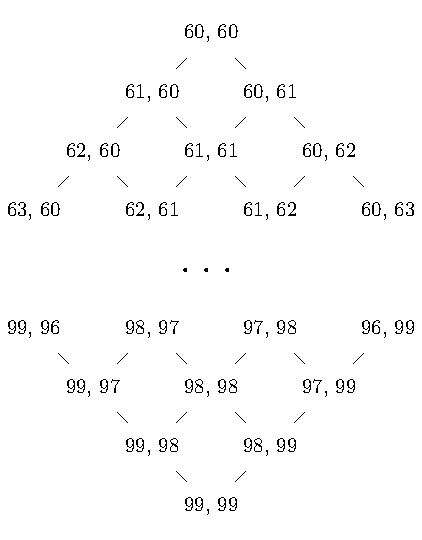
\includegraphics[width=.4\linewidth]{img/training_scheme.pdf}
			\caption{
				The possible ways to train from 60 attack and strength to 99 attack and strength. Branching to the left represents training an attack level, and to the right is strength. At a point, 99 is reached along the edge and the tree cannot grow out anymore and eventually collapses to the desired levels.
			}\label{fig:training_scheme}
		\end{figure}

		The optimization task then becomes how do we traverse from the top of this tree-like structure to the bottom most efficiently? We can assign a \emph{cost} to each edge in this graph corresponding to the time it takes to level up. The experience required to level up to a given level, $x$ is:
		\begin{equation}
			\xi(x) = \frac{\left \lfloor x - 1 + 300\times 2^\frac{(x-1)}{7} \right \rfloor}{4}
		\end{equation}
		The time to level attack or strength is given respectively by,
		\begin{align}
			t^{\text{attack}} &= \xi(a) / \langle E(a, s; \text{attack}) \rangle \\
			t^{\text{strength}} &= \xi(s) / \langle E(a, s; \text{strength}) \rangle,
		\end{align}
		where we explicitly show that the experience per hour, E depends on the attack style (due to the combat bonus). The above two equations give the cost for branching to the left, and right, respectively. There is a relatively simple pattern to generate the children of any row. Building the whole tree has a \textcolor{red}{$\mathcal{O}( (A-a)(S-s) )$ time-complexity}, making this a feasible operation. The sum of costs (times) along any path is the time it takes to complete the leveling. Minimizing this corresponds to the family of problems called shortest path problems. Our particular problem is solving the single-source directed graph with non-negative weightings. This can be solved using the \href{https://en.wikipedia.org/wiki/Dijkstra%27s_algorithm}{Dijkstra Algorithm} in quadratic time. A Python library \href{https://pypi.org/project/Dijkstar/}{Dijkstra} implements this. So this problem is solved in two parts: 1) Construct graph, 2) Apply Dijkstra. A few solutions are shown in Fig.~\ref{fig:levels_recur}. There is occasional switching, but ultimately strength is maximized first, followed by attack.

		\begin{figure}[H]
			\centering
			\begin{subfigure}{\textwidth}
				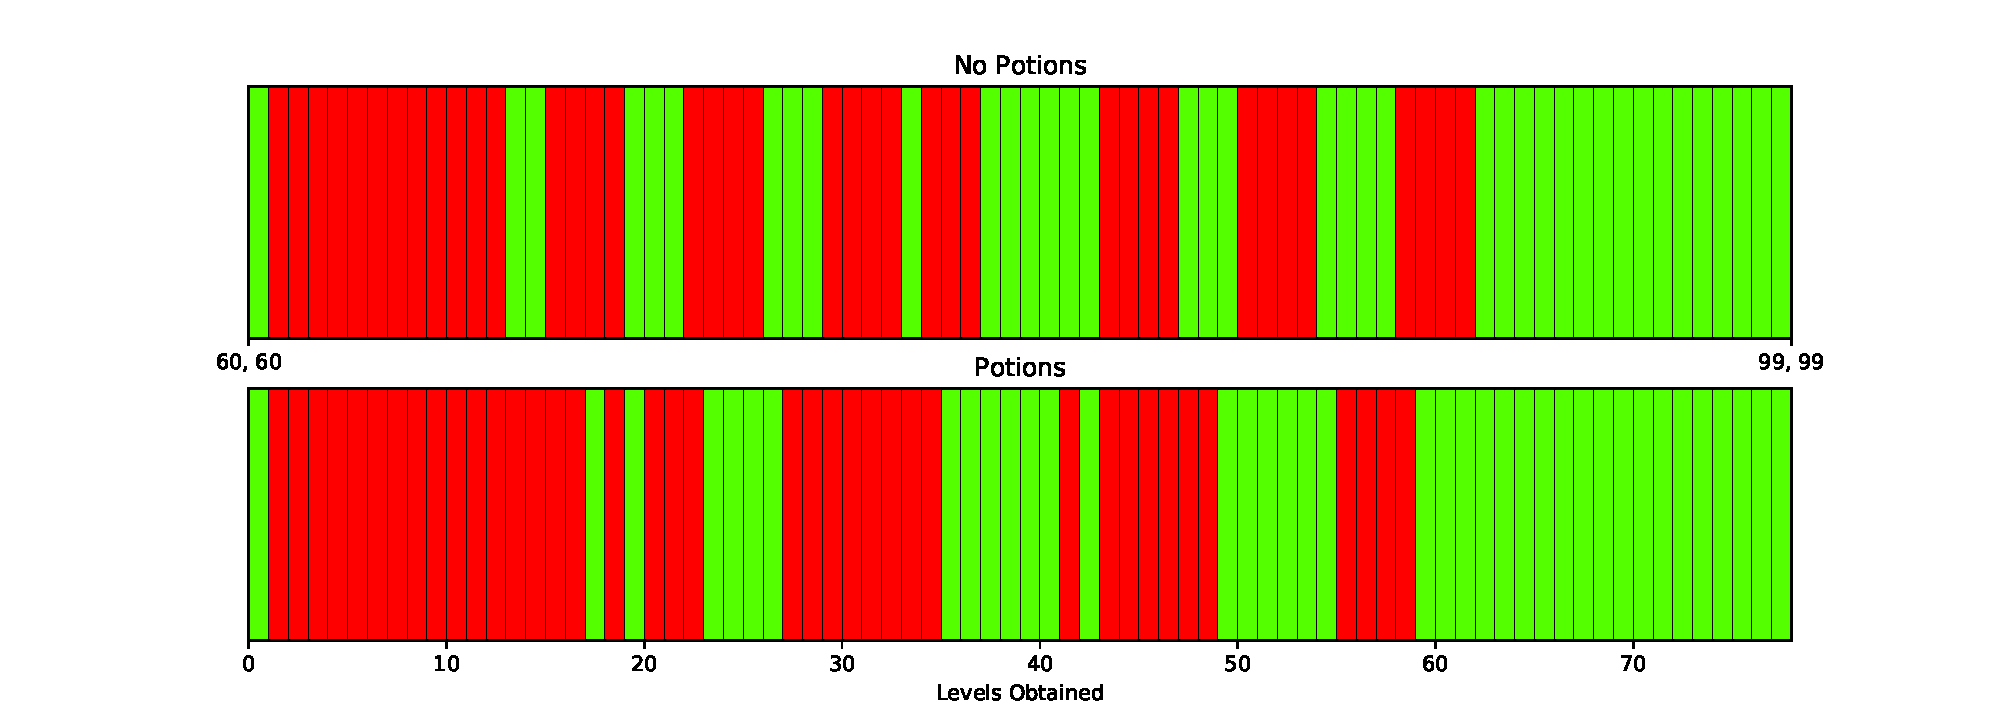
\includegraphics[width=\linewidth]{img/levels_recur.pdf}
			\end{subfigure}
			\begin{subfigure}{\textwidth}
				\includegraphics[width=\linewidth]{img/levels_recur_60_90.pdf}
			\end{subfigure}
			\begin{subfigure}{\textwidth}
				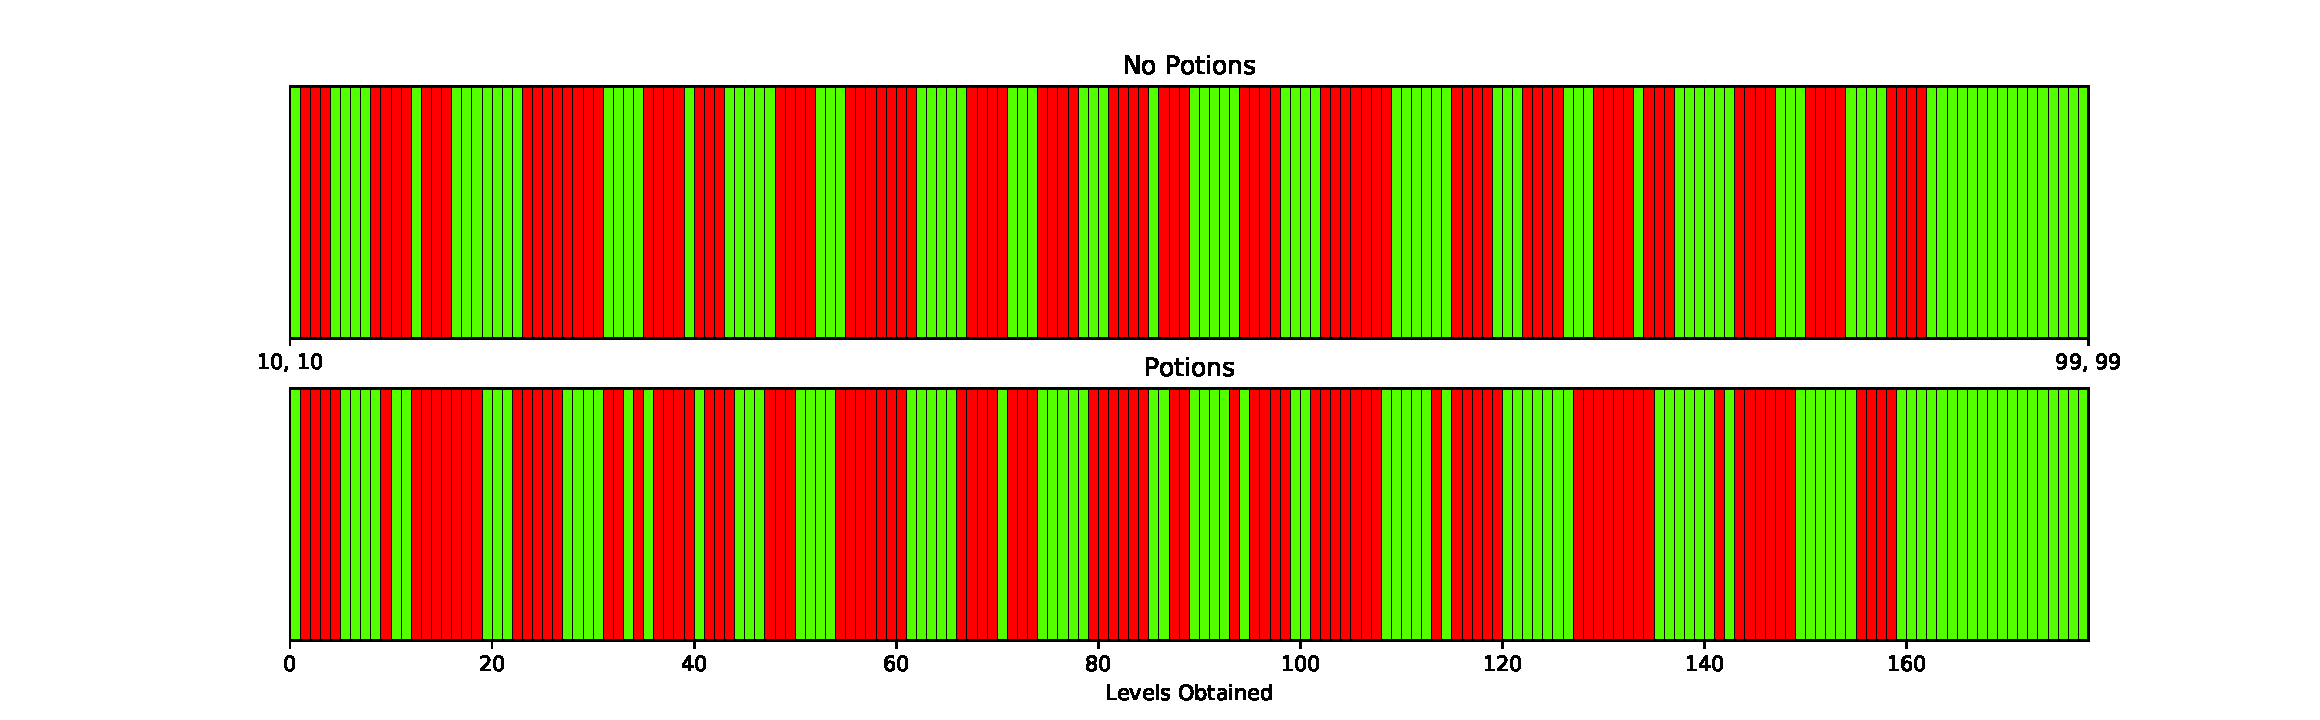
\includegraphics[width=\linewidth]{img/levels_recur_10_10.pdf}
			\end{subfigure}
			\caption{
				The most efficient training is obtained by following these training schemes. Starting on the left, the player should train attack (green) or strength (red) until they reach the right side (99 attack & strength).
				Three schemes are shown for different starting levels: (60, 60), (60, 90), and (10, 10). The latter is unrealistic since 60 attack is required to wield the dragon scimitar used in these calculations, but this shows the long term behavior. Additionally, for each scheme calculations using or not using potions is shown.
			}\label{fig:levels_recur}
		\end{figure}


		\begin{figure}[H]
			\centering
			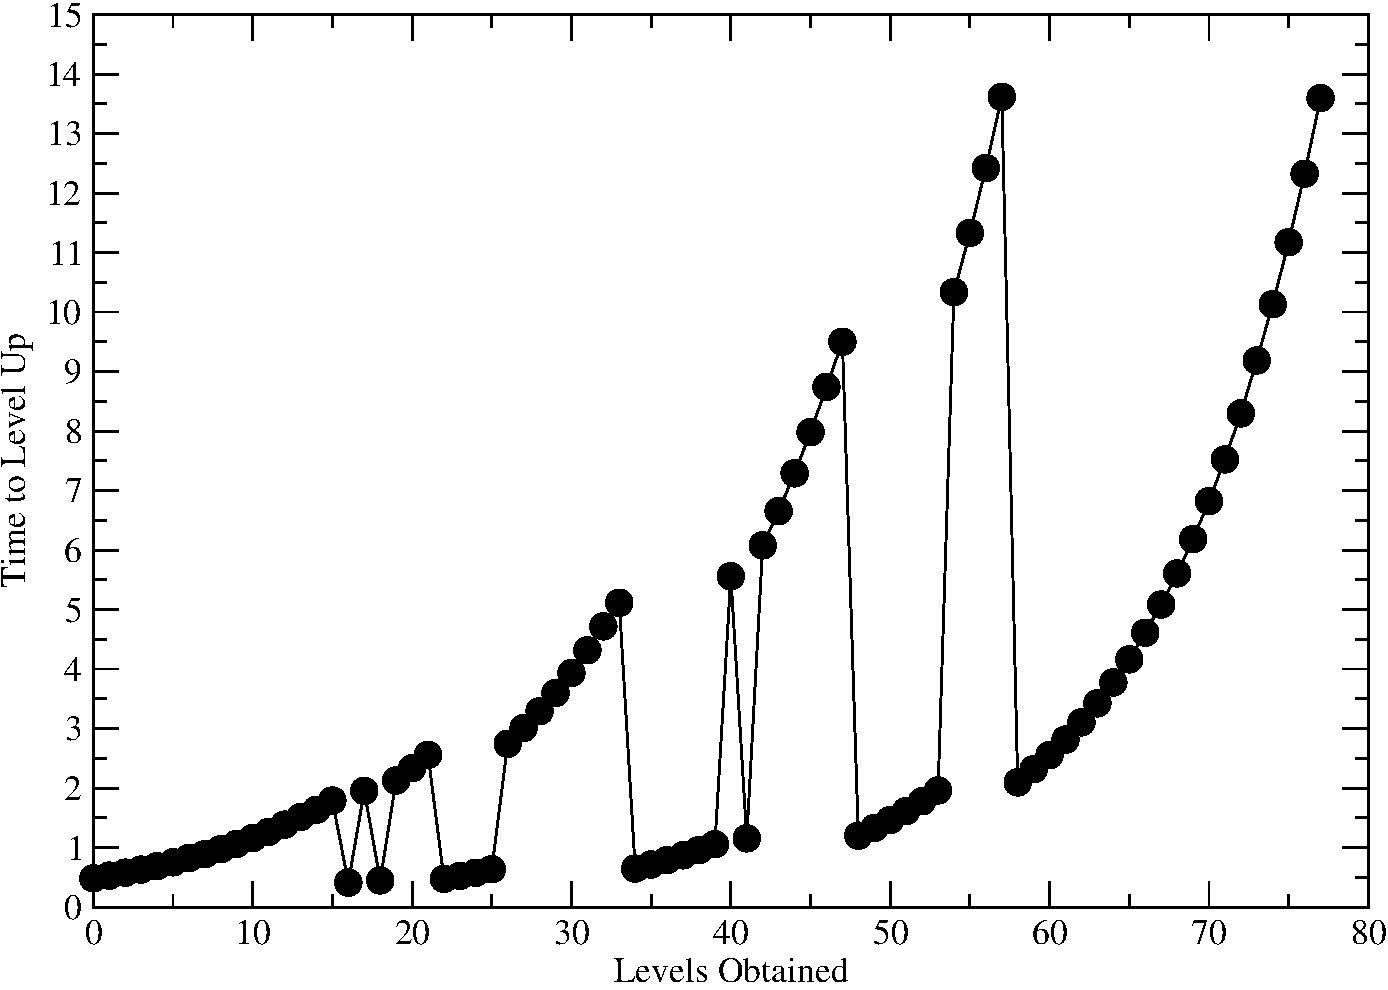
\includegraphics[width=\linewidth]{img/fig_time.pdf}
			\caption{
				Following the optimal training scheme (using potions) starting from (60, 60), the training time for each level is plotted until the player arrives at (99, 99).
			}\label{fig:time}
		\end{figure}

		Taking one of these schemes, like $(60, 60)\to(99, 99)$ using potions, we can calculate the actual time required to move to each next ``strip'' in Fig.~\ref{fig:levels_recur}, as done in Fig.~\ref{fig:time}. Strength is often trained first resulting in training times that are higher earlier on. Because of this, training is switched to attack. There are actually two competing effects at play. Attack has a small bonus to dps, but is often a lower level and is therefore easier to obtain. Conversely, strength has a large bonus, but quickly becomes too time-expensive to train before any benefit is received, so briefly attack is trained. After 99 strength is obtained $~$$60$ levels, attack is the only thing left to train until max. If the scheme was to alternate levels between attack and strength, the curve would be a single curve, but this staggered scheme results the prominent bifurcation.

	\chapter{Improvements}
		Health regeneration. Analytic solution? Constant Combat (acts as reduced weapon speed so multiplicative). Health Sustainability. The last two shouldn't impact rankings since they are multiplicative and independent of the calculation method. Based on this, we can say that exact rankings is more important than exact approximations for practical purposes. Is the treatment $h=1$ for a kill valid for all methods? Since crude and Bitterkoekje can get to 0? I've seen (enemy) hp go up in under a minute. There must be a global timer, not just every 60s after you drop below max health.

	\chapter{Conclusion}
		We summarized the combat mechanics behind effective levels, accuracy, and maximum hits. We performed detailed calculations to determine piecewise average damage, based on whether overkill was present. In contrast to the Bitt-Nuke model, we maintain this piecewise relation and evaluate an recursive scheme to determine a more accurate form for the average damage. An analytic approximation was used to handle non-integer turns to kill an opponent, which can ultimately be used to calculate experience per hour. We discuss the effects which are not considered like health regeneration, and constant combat. Finally, experience per hour models are compared. The Recursive model is the best model due to its accuracy, and since it satisfies the expected upper bound property. Future work may look into forming an optimization problem.





		\newpage
		\begin{appendices}
		% \appendix
		% \titleformat{\section}[display]{\normalfont\Large\bfseries}{\appendixname\enspace\thesection}{.5em}{}
		% \titleformat{\chapter}[display]{\normalfont\Large\bfseries}{\appendixname\enspace\thesection}{.5em}{}
		\chapter{Average Damage}\label{app:average_damage}

			The average damage described in Section \ref{sec:average_damage} can be expanded to give,
			\begin{align}
				\langle D \rangle_\text{overall} &= \frac{1}{h_0}\left(
					\sum_{n=M+1}^{h_{0}}\frac{M}{2} +
					\sum_{n=1}^{y} \frac{n}{2}\left(2 - \frac{n + 1}{M+1}\right)
				\right) \\
				&= \frac{1}{h_0}\left(
					\frac{M}{2}(h_0-y) +
					\sum_{n=1}^{y}n - \frac{1}{2}\sum_{n=1}^yn\frac{n + 1}{M+1}
				\right) \\
				&= \frac{1}{2h_0}\left(
					Mh_0-My + y(y+1)
					 - \frac{1}{2({M+1})}\sum_{n=1}^y(n^2 + n)
				\right) \\
				&= \frac{1}{2h_0}\left(
					Mh_0-My + y(y+1) - \frac{y(y+1)}{2({M+1})}
					 - \frac{y(n+1)(2y+1)}{6({M+1})}
				\right) \\
				&= \frac{1}{2h_0({M+1})}\left(
					M^{2}h_{0}-M^{2}y+My^{2}+yM+Mh_{0}-My - \frac{y^3-y}{3}
				\right) \\
				&= \frac{y(y+1)}{h_0({M+1})}\left(
					\frac{M(M+1)h_{0}}{2y(y+1)}+\frac{(y-M)M}{2(y+1)} - \frac{y-1}{6}
				\right) \\
				&= \frac{y(y+1)}{h_0({M+1})}\left(
					\frac{M(M+1)h_{0}}{2y(y+1)}+\frac{(y-M)M}{2(y+1)} +\frac{y+1}{2} -\frac{1}{3}(2y+1)
				\right)
				\label{eq:app-average-damage-original}
			\end{align}
			where $y=\min(M, h_0)$. In the second line, we used:
			\begin{align}
				\sum_{a+1}^b1&=\begin{cases}
						b-a&\text{ if } b>a\\
						0 &\text{ else }
					\end{cases}\\
					&=b-\begin{cases}
						a &\text{ if } b>a\\
						0 &\text{ else }
					\end{cases}\\
					&=b-\min(a, b)
			\end{align}
			To finish, let's focus on,
			\begin{align}
				 &\frac{M(M+1)h_{0}}{2y(y+1)}+\frac{(y-M)M}{2(y+1)} +\frac{y+1}{2} \\
				=&\frac{1}{2y(y+1)}\Big[ M(M+1)h_{0}+y(y-M)M +y(y+1)^2 \Big]\\
				=&\frac{1}{2y(y+1)}\Big[ M^2h_{0}+Mh_0+My^2-M^2y +y^3+2y^2+y \Big].\label{eq:app-average-damage-bracket}
			\end{align}
			This is a hard equation to simplify since the $M$'s and $h_0$'s are implicitly embedded in the $y$'s, but if you play with it long enough you can ``discover'' a way to simplify it - a form \textit{power reduction} that relies on getting rid of as many $y$'s as possible.

			\section{Power Reduction}
				I'd like to preface the next part by saying the final result can easily be determined by plugging in $m$ as the $\min$, and $h_0$ as the $\min$ and combining the result. In this instance it works out nicely, but we will focus on general machinery to solve these problems assuming the solution was not so nice. Our goal here is to pull the $m$'s and $h_0$'s out of $y$. To do this, let's see if there is a way to construct $y^2$ from the other variables, specifically only using $y^1$. We know that if $M < h_0$, we need a term like $M^2$, and in the opposite case, we need a term like $h_0^2$,
				\begin{align}
					y^2 \sim M^2 \text{ or } h_0^2.
				\end{align}
				Based on this, we should be able to use $\min$ to switch between these two. So if we write the first term using $y$, we'd have something like $My$, which is true when $M$ is the minimum. If it isn't the minimum, there should be a second term which cancels the now $Mh_0$ term plus the required $h_0^2$ term:
				\begin{align}
					y^2 = My + h_0(y - M)\,\,\,\,\,(!)
				\end{align}
				Using the same logic, we can inductively deduce,
				\begin{align}
					\boxed{y^{n+1} = My^n + h_0^n(y - M) = My^n + h_0^ny - Mh_0^n.}
				\end{align}
				(and as an identity for the math people, with $\gamma = \min(a, b)$):
				\begin{align}
					\boxed{\gamma^{n+1} = a\gamma^n + b^n(\gamma - a) = a\gamma^n + b^n\gamma - ab^n}
				\end{align}
				In fact, this holds for $\max$ as well, or any \emph{similar} piece-wise function.
				Writing this as a recursive sequence by letting $g(n)=\gamma^n$ yields,
				\begin{align}
					g(n+1) = ag(n) + b^n(g(1) - a),
				\end{align}
				Under the initial condition $g(1)=\gamma$, \href{https://www.wolframalpha.com/input/?i=g%28n%2B1%29%3Da*g%28n%29%2Bb%5En%28C-a%29}{WolframAlpha} gives the general solution as,
				\begin{align}
					g(n) = a^n + (\gamma - a)\frac{a^n - b^n}{a - b} \\
					\boxed{g(n) = a^n + (\gamma - a)\sum_{i=0}^{n-1} a^{n-i-1}b^j,}
				\end{align}
				where the second line uses the difference of powers formula. This could have been solved by hand, but we've had enough fun with recursion in the other sections! This yields,
				\begin{align}
					g(1) &= \gamma\\
					g(2) &= a^2 + (\gamma - a)(a + b) \\
						&= a^2 + a\gamma - a^2  + b\gamma - ab \\
						&= a\gamma + b(\gamma - a) \\
					g(3) &= a^3 + (\gamma - a)\frac{a^3 - b^3}{a - b} \\
						&= a^3 + (\gamma - a)(a^2 + ab + b^2) \\
						&= a^3 + \gamma a^2 + \gamma ab + \gamma b^2 - a^3 - a^2b - ab^2 \\
						&= \gamma a^2 + \gamma ab + \gamma b^2 - a^2b - ab^2.
				\end{align}
				These agree with the original iterative equation. Okay, so this is a bit overkill since at most $y^3$ appears, so having general powers isn't too helpful. Nonetheless, we can now reduce the powers of $y$ in the original equation, and see how that simplifies things.
			\section{Simplifying}
				We can now reduce the bracketed term in Eq.~\ref{eq:app-average-damage-bracket}:
				\begin{align}
				 	&\phantom{=}M^2h_0+Mh_0+My^2                   -M^2y + y^3                                    +2y^2+y \\
				 	&=M^{2}h_{0}+Mh_{0}+M^{2}y+h_{0}yM-h_{0}M^{2}-M^{2}y+yM^{2}+yMh_{0}+yh_{0}^{2}+\\
				 		&\phantom{=========} -M^{2}h_{0}-h_{0}^{2}M+2My+2h_{0}y-2h_{0}M+y\\
				 	&=\left(-M^{2}y+yM^{2}+M^{2}y+yMh_{0}+yh_{0}^{2}+2My+2h_{0}y+y+h_{0}yM\right)+\\
				 		&\phantom{=========} \left(M^{2}h_{0}+Mh_{0}-h_{0}M^{2}+-M^{2}h_{0}-h_{0}^{2}M-2h_{0}M\right)\\
				 	&=\left(2My+2h_{0}y+y+2yMh_{0}+M^{2}y+yh_{0}^{2}\right)+\left(-M^{2}h_{0}-h_{0}^{2}M-h_{0}M\right)
				\end{align}
				Having eliminated the ``hidden'' variables, let's try to re-group into powers of $y$:
				\begin{align}
				 	&=y^{2}+\left(My+h_{0}y+y+2yMh_{0}+M^{2}y+yh_{0}^{2}\right)+\left(-M^{2}h_{0}-h_{0}^{2}M\right)\\
				 	&=2y^{2}+y+2yMh_{0}+M^{2}y+yh_{0}^{2}+-M^{2}h_{0}-h_{0}^{2}M+Mh_{0}\\
				 	&=y^{2}M+y+y^{2}+y^{2}h_{0}+y^{2}+Mh_{0}\\
				 	&=y\left(yM+yh_{0}+y+M+h_{0}+1\right)\\
				 	&=y\left(y+1\right)\left(M+h_{0}+1\right)
				\end{align}
				Putting this into the corresponding term in Eq.~\ref{eq:app-average-damage-original} gives
				\begin{align}
					\frac{1}{2y(y+1)}y(y+1)\left(M+h_{0}+1\right) = \frac{1}{2}\left(M+h_{0}+1\right)
				\end{align}
				and so finally we arrive at,
				\begin{align}
					\boxed{\langle D \rangle_\text{overall} = \frac{y(y+1)}{h_0({M+1})}\left[
						 \frac{1}{2}\left(M+h_{0} + 1\right) -\frac{1}{3}(2y+1)
					\right]}.
				\end{align}
		\newpage
		\chapter{Analytic Form Attempt}\label{app:analytic_form_attempt}
			Here we will attempt to derive a more useful form of Eq.~\ref{eq:recur}. We will start with a slightly simpler relation,
			\begin{align}
				h_{n+1} &= h_n^2 + h_n.
			\end{align}
			We note that in general, this will be an expansion in terms of $h_0$,
			\begin{align}
				h_n = \sum_{i=1}^m a_i h_0^i.
			\end{align}
			Our goal then, is to determine the set of coefficients ${a_i}$. These coefficients implicitly depend on $n$. Our next iteration will look like,
			\begin{align}\label{eq:sum_n+1th_term}
				h_{n+1} = \left(\sum_{i=1}^m a_i h_0^i\right)^2 + \sum_{i=1}^m a_i h_0^i.
			\end{align}
			The squared term is actually very messy to deal with, requires the use of the Multinomial Theorem which (for the specific case $p=2$) states,
			\begin{align}
				\left(\sum_{i=1}^m x_i\right)^2 = 2\sum_{\{k_m\}=2} \prod_{t=1}^m \frac{x_t^{k_t}}{k_t!},
			\end{align}
			where $\{k_m\}=2$ denotes the sets of $m$ integers which add to two. For $m=4$ one example might look like: $(1, 0, 0, 1)$. For those of you familiar with this, these sets arise from integer partitioning, but we won't go over how these are generated, but just know there are algorithms for generating them. We will drop the $=2$ portion for brevity. Our form can be obtained with the transformation $x_i\to a_ih_0^i$,
			\begin{align}
				\left(\sum_{i=1}^m a_ih_0^i\right)^2 &= 2\sum_{\{k_m\}} \prod_{t=1}^m \frac{a_t^{k_t} h_0^{tk_t}}{k_t!} \\
				&= 2\sum_{\{k_m\}} \prod_{t=1}^m \frac{a_t^{k_t}}{k_t!} h_0^{\sum_{t=1}^m tk_t}.
			\end{align}
			Now let's return to the general n'th term (Eq.~\ref{eq:sum_n+1th_term}),
			\begin{align}
				h_n = 2\sum_{\{k_m\}} \prod_{t=1}^m \frac{a_t^{k_t}}{k_t!} h_0^{\sum_{t=1}^m tk_t} + \sum_{i=1}^m a_i h_0^i.
			\end{align}
			As-is, these cannot be combined. To handle this, we impose an ordering on $\{k_m\}$ so they they are given in increasing values of $\sum tk_t$, we will denote this as $\{k_m\}_i^{L}\uparrow$, where $L$ indicates the sum's value for the current set, and $i$ is the index of the current set. Now,
			\begin{align}
				h_n = 2\sum_{\{k_m\}_i^L\uparrow} \prod_{t=1}^m \frac{a_t^{k_t}}{k_t!} h_0^{L_m} + \sum_{i=1}^m a_i h_0^i.
			\end{align}
			Our only hope of combining these terms is to match up the powers. The good news is that now each term on the left, and right correspond to a single power.
			\begin{align}
				h_n = 2\sum_{\{k_m\}_i^L\uparrow} \left(\prod_{t=1}^m \frac{a_t^{k_t}}{k_t!} + a_i \right) h_0^{L_m},
			\end{align}
			Now, we should start from the bottom ($n=0$) and see if we can build up. For $n=0$, $h_{1}=h_0^2+h_0$. So the coefficients are $\{a\}^1 = (1, 1, 0, 0, 0, ...)$, where the zero padding accounts for the fact that the powers on the linear sum are less than the powers on the quadratic sum.

			We can read off the coefficient is we sort-of invert the sum notation. Let's instead sum across $i$.
			\begin{align}
				h_n = 2\sum_{i} \left(\prod_{\{k_t\}_i}^m \frac{a_t^{k_t}}{k_t!} + a_i \right) h_0^{L_i}.
			\end{align}
			Now the coefficient for the $L_i$'th power for the next iteration is
			\begin{align}
				a_{L_i} = 2\left(\prod_{\{k_t\}_i}^m \frac{a_t^{k_t}}{k_t!} + a_i \right).
			\end{align}
			This actually works out really well since the coefficients for our original problem simply get multiplied by $\gamma$! Let's make another simplification by letting $k_t$ be represented by a vector, $\vec k$ and constructing respective operations,
			\begin{align}
				a_{i, n+1} = 2 \frac{\boldsymbol{a}_n^\boldsymbol{k_i}}{\boldsymbol{k_i}!} + 2a_{i, n}.
			\end{align}
			Here a vector to the power of a vector is the product of the element-wise powers, and the factorial of a vector is the product of the element-wise factorials. This isn't very useful since it still requires an iterative scheme.
		% \end{appendices}
		\newpage
		\chapter{Recursive Approximation Justification}\label{app:recursive_approximation_justification}
			We begin with Eq.~(\ref{eq:simplified_recursion}) which we will restate here with $h_m\to x_n$:
			\begin{align}
				x_{n+1} = x_n - \frac{x_n}{2}\left(2 - \frac{x_n + 1}{M+1} \right).
			\end{align}
			This formulation looks similar to Newtons method for finding the root of $f(x)$, which is given as
			\begin{align}
				x_{n+1} = x_n - \frac{f(x_n)}{f'(x_n)}.
			\end{align}
			After some algebra we find that,
			\begin{align}
				\frac{f(x_n)}{f'(x_n)} = x_n(1-\gamma x_n).
			\end{align}
			This can be easily solved for $f(x)$ since this is a separable equation:
			\begin{align}
				\frac{df}{f} &= \frac{dx}{x(1-\gamma x)} \\
				\int \frac{df}{f} &= \int \frac{dx}{x(1-\gamma x)} \\
				\ln(f) &= \ln|x| - \ln|\gamma x - 1| + C \\
				f(x) &= e^C |x||\gamma x - 1|
			\end{align}
			The error, $\epsilon$ in the next iteration of Newtons method is given as,
			\begin{align}
				\epsilon_{n+1} = \epsilon_{n}^2 \left | \frac{f''(r)}{2f'(r)} \right |,
			\end{align}
			where $r$ is the root we desire. In this case the root we want is,
			\begin{align}
				\lim_{n\to\infty} x_n = 0
			\end{align}
			since this corresponds to the health reaching zero. The ratio becomes,
			\begin{align}
				\left| \frac{f''(r)}{2f'(r)} \right| = \gamma,
			\end{align}
			which simplifies the error equation to,
			\begin{align}
				\epsilon_{n+1} = \gamma \epsilon_{n}^2.
			\end{align}
			This is exactly the same recursive equation we had before! Except that now we have error in health instead of health. So how does this connect? Since we already know the root value (which is 0), the error becomes the upper bound on the health. This means that if we have an error of, for example, 1 that the health must be below that. So, by solving $\epsilon=h$ we can find the number of iterations required to reach below that health. This solution is already given earlier but in the context of error we have,
			\begin{align}
				\epsilon_{n} = \frac{1}{\gamma}\left( \frac{1}{2} - \gamma \right)^{2^{n}} \\
				n = \log_2 \log_{\frac{1}{2} - \gamma} (\gamma \epsilon).
			\end{align}
			This has done two things: justify the use exclusion of the $h_m$ term in the original recursive equation (instead of excluding $h^2_m$), and provided a second interpretation of the meaning of $h = 1$. The error comes from a Taylor series, but interestingly all higher order terms die off so this is actually exact. This suggests that for higher precision, the assumption that $\epsilon$ is small is violated and the Taylor series formulation no longer holds.

		\end{appendices}

\end{document}



% \documentclass[tikz, margin=0mm]{standalone}
% % a more complicated graph using tkz-graph
% % depending on the actual graph this could be partially automated
% % with tikz \for loops
% \usepackage{tkz-graph}
% \usetikzlibrary{calc}
% \renewcommand*{\EdgeLineWidth}{0.15pt}

% \begin{document}
% \begin{tikzpicture}
%     \GraphInit[vstyle=Empty]
%         \Vertex[x=1,y=5-2,L={60, 60}]{X}
%         \Vertex[x=0,y=5-3,L={61, 60}]{A}
%         \Vertex[x=2,y=5-3,L={60, 61}]{B}
%         \Vertex[x=-1,y=5-4,L={62, 60}]{C}
%         \Vertex[x=1,y=5-4,L={61, 61}]{D}
%         \Vertex[x=3,y=5-4,L={60, 62}]{E}

%         \Vertex[x=-2,y=5-5,L={63, 60}]{F}
%         \Vertex[x=0,y=5-5,L={62, 61}]{G}
%         \Vertex[x=2,y=5-5,L={61, 62}]{H}
%         \Vertex[x=4,y=5-5,L={60, 63}]{I}
%     \Edges(A,X,B)
%     \Edges(C,A,D,B,E)
%     \Edges(F,C,G,D,H,E,I)

%     \node at (1, -1) {\Huge \ldots};

%     \GraphInit[vstyle=Empty]
%         \Vertex[x=1,y=-3+-2,L={99, 99}]{X}

%         \Vertex[x=0,y=-1+-3,L={99, 98}]{A}
%         \Vertex[x=2,y=-1+-3,L={98, 99}]{B}

%         \Vertex[x=-1,y=1+-4,L={99, 97}]{C}
%         \Vertex[x=1,y=1+-4,L={98, 98}]{D}
%         \Vertex[x=3,y=1+-4,L={97, 99}]{E}

%         \Vertex[x=-2,y=3+-5,L={99, 96}]{F}
%         \Vertex[x=0,y=3+-5,L={98, 97}]{G}
%         \Vertex[x=2,y=3+-5,L={97, 98}]{H}
%         \Vertex[x=4,y=3+-5,L={96, 99}]{I}
%     \Edges(A,X,B)
%     \Edges(C,A,D,B,E)
%     \Edges(F,C,G,D,H,E,I)

% \end{tikzpicture}
% \end{document}